\input{../../.preambles/01-semester_work}
\input{../../.preambles/10-russian}
\input{../../.preambles/20-math}
\input{../../.preambles/22-vectors}
\input{../../.preambles/30-physics}

\newcommand{\ds}{\displaystyle}

\begin{document}
\maketitlepage{Факультет электроники и вычислительной техники}{физики}
{Электродинамика}{студент группы Ф-369\\Чечеткин~И.~А.}
{доцент Грецов~М.~В.}{№3}

Задача 1.15: \emph{Определить поле, создаваемое заряженным проводящим шаром
радиуса \( a \). Заряд его \( Q \). Диэлектрическая проницаемость окружающей
среды \( \eps = \eps(r) \), где \( r \) -- расстояние от центра шара.}

\vspace*{2em}
\emph{Решение:}

\begin{minipage}{.4\textwidth}
    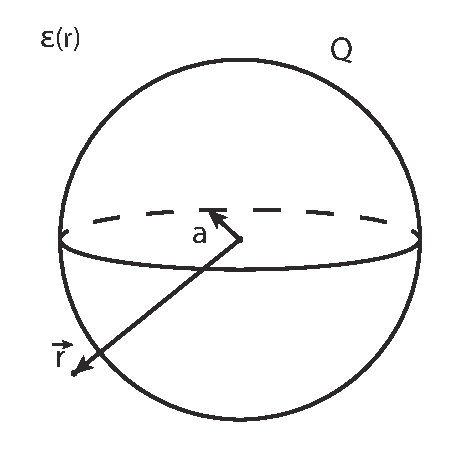
\includegraphics[width=\textwidth]{electric_ball}
\end{minipage}
\begin{minipage}{.55\textwidth}
Учитывая, что задача имеет сферическую симметрию, воспользуемся для решения
сферической системой координат. Тогда можно записать следующие соотношения:
\[
	D_r = D(r), \quad D_\theta = D_\psi = 0.
\]

Запишем уравнение Максвелла для индукции электрического поля:
\( \div{\vec{D}} = \rho \).
\end{minipage}

Воспользовавшись теоремой Остроградского-Гаусса, имеем:
\[
	\int \div\vec{D}\,dV = \oint \vec{D}\d\vec{S} = D \oint dS = 4\pi r^2 D; \quad
	\int \rho\,dV = q.
\]

Поле внутри шара, то есть при \( r < a \) и \( q = 0 \):
\[
	D = E = 0.
\]

Поле вне шара, то есть при \( r > a \) и \( q = Q \):
\[
	D = \frac{Q}{4\pi r^2}; \quad
	E = \eps\Ezero D = \frac{Q}{4\pi\Ezero\eps(r) \cdot r^2}.
\]

\vspace*{2em}   
\emph{Ответ:} \( \ds D = \frac{Q}{4\pi r^2}, \quad
E = \frac{Q}{4\pi\Ezero\eps(r) \cdot r^2} \).

\newpage
%-------------------------------------------------------------------------------
Задача 1.59: \emph{Вычислить емкость плоского конденсатора. Поверхность
обкладок \( S \), между ними два плоскопараллельных слоя однородных
диэлектриков. Толщина первого слоя \( d_1 \), проницаемость \( \eps_1 \),
второго -- соответственно \( d_2 \) и \( \eps_2 \). Краевым эффектом
пренебречь.}

\vspace*{2em}
\emph{Решение:}

\begin{minipage}{.4\textwidth}
    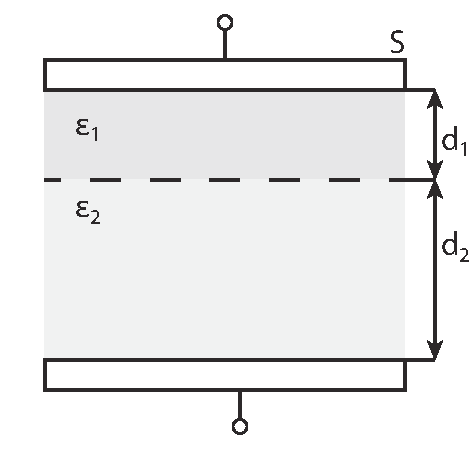
\includegraphics[width=\textwidth]{capacitor}
\end{minipage}
\begin{minipage}{.55\textwidth}
По определению емкости плоского конденсатора:
\( \ds C = \frac{q}{\Delta\phi} = \frac{q}{Ed} = \frac{\sigma S}{Ed} \).

Окружим малый участок пластины замкнутой цилиндрической поверхностью.
Запишем теорему Гаусса для \( \vec{D} \):
\[
    \oiint\limits_S \vec{D}\d\vec{S} = \sigma S_{\emph{тор}_H}.
\]

Интеграл в правой части можно расписать следующим образом:
\end{minipage}
\[
    \oiint\limits_S \vec{D}\d\vec{S} = \iint\limits_{S_\emph{бок}} \vec{D}
    \d\vec{S} + \iint\limits_{S_{\emph{тор}_H}} \vec{D}\d\vec{S} +
    \iint\limits_{S_{\emph{тор}_B}} \vec{D}\d\vec{S}.
\]

Так как вне конденсатора поля нет, то \( \ds \iint\limits_{S_{\emph{тор}_B}}
\vec{D}\d\vec{S} = 0 \), а так же поскольку поле \( \vec{D} \) в этом цилиндре
направлено от одной обкладки к другой, перпендикулярно ей, то, следовательно,
\( \ds \iint\limits_{S_\emph{бок}} \vec{D}\d\vec{S} = 0 \).

Тогда \( \ds
    \sigma S_{\emph{тор}_H} = \iint\limits_{S_{\emph{тор}_H}} \vec{D}\d\vec{S} =
    D\iint\limits_{S_{\emph{тор}_H}} dS = DS_{\emph{тор}_H}
\), откуда \( D = \sigma = \eps\Ezero E\).

Тогда емкость:
\( \ds
    C = \frac{\sigma S}{Ed} = \frac{\eps\Ezero ES}{Ed} = \frac{\eps\Ezero S}{d}
\).

Для вычисления емкости двухслойного конденсатора представим его в виде
последовательного соединения двух однослойных, емкости которых:
\[
    C_1 = \frac{\eps_1\Ezero S}{d_1}, \quad C_2 = \frac{\eps_2\Ezero S}{d_2}.
\]

Тогда:
\( \ds
    C = \frac{C_1C_2}{C_1 + C_2} = \frac{\eps_1\eps_2\Ezero^2 S^2}
    {S\Ezero d_1d_2\left(\frac{\eps_1}{d_1} + \frac{\eps_2}{d_2}\right)} =
    \frac{\Ezero\eps_1\eps_2 S}{\eps_1d_2 + \eps_2d_1}
\).

\emph{Ответ:} \( C = \cfrac{\Ezero\eps_1\eps_2 S}{\eps_1d_2 + \eps_2d_1} \).

\pagebreak
%-------------------------------------------------------------------------------
Задача 1.116: \emph{Найти распределение зарядов, индуцированных на поверхности
цилиндра предыдущей задачи, и суммарный заряд, индуцированный на единице длины
цилиндра.}
\vspace*{-1em}

\singlespacing
{\footnotesize\emph{Предыдущая задача: В вакууме имеется бесконечно длинный заземленный
проводящий круглый цилиндр радиуса \( a \). Параллельно его оси протянута нить на
расстоянии \( l > a \) от нее. Нить равномерно заряжена с линейной плотностью
\( \chi \). Определить создаваемое ею поле и силу, действующую на единицу длины
нити.}}

\vspace*{1em}
\onehalfspacing
\emph{Решение:}

Из решения задачи 1.115:
\[
    E_R = -\pder{\phi}{R} = 2\chi \Biggl(\frac{R - l\cos\theta}{R_1^2} -
    \frac{R - l'\cos\theta}{R_2^2}\Biggr),
\]
где \( R_1 = \sqrt{l^2 + R^2 - 2lR\cos\theta} \), \( R_2 = \sqrt{l'^2 + R^2 -
2l'R\cos\theta} \), \( l' = a^2/l \).

Распределение заряда на поверхности определяется формулой:
\begin{gather*}
    \sigma = -\Ezero\pder{\phi}{R}\biggr|_{R = a} = \Ezero E_R\bigr|_{R = a} =
    2\chi\Ezero\Biggl(\frac{R - l\cos\theta}{l^2 + R^2 - 2lR\cos\theta} - \\ -
    \frac{R - a^2/l\cos\theta}{a^4/l^2 + R^2 - 2a^2R/l\cos\theta}\Biggr)_{R = a}
    = 2\chi\Ezero\Biggl(\frac{a - l\cos\theta}{l^2 + a^2 - 2al\cos\theta} - \\ -
    \frac{a - a^2/l\cos\theta}{a^4/l^2 + a^2 - 2a^3/l\cos\theta}\Biggr) =
    2\chi\Ezero\Biggl(\frac{a^2-al\cos\theta}{a(a^2 + l^2 - 2al\cos\theta)} - \\
    - \frac{l^2 - al\cos\theta}{a(a^2 + l^2 - 2al\cos\theta)}\Biggr) =
    2\chi\Ezero\frac{a^2 - l^2}{a(a^2 + l^2 - 2al\cos\theta)}.
\end{gather*}

Суммарный заряд, индуцированный на единице длины цилиндра, можно выразить через
поверхностную плотность зарядов следующим образом:
\[
    q_\emph{и} = \int \sigma\,dS = \int\limits_0^{2\pi} a\sigma\d\theta =
    2\chi\Ezero \int\limits_0^{2\pi} \frac{a^2 - l^2}{a^2 + l^2 -
    2al\cos\theta}\d\theta = 2\chi\Ezero\cdot (-2\pi) = -4\pi\Ezero\chi.
\]

\vspace*{2em}
\emph{Ответ:} \( \sigma = \cfrac{2\chi\Ezero(a^2 - l^2)}{a(a^2 + l^2 -
2al\cos\theta)} \), \( q_\emph{и} = -4\pi\Ezero\chi \).

\newpage
%-------------------------------------------------------------------------------
Задача 2.35: \emph{Полупространство заполнено однородным магнетиком с
проницаемостью \( \mu_1 \), а второе полупространство -- однородным магнетиком
с проницаемостью \( \mu_2 \). В первой среде имеется плоский контур \( L \) с
током \( I \), расположенный параллельно плоскости раздела обеих сред на
расстоянии \( h \) от нее. Определить создаваемое током магнитное поле.}

\vspace*{2em}
\emph{Решение:}

\begin{figure}[h!]
	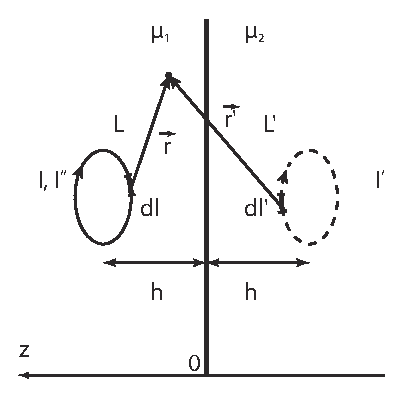
\includegraphics[width=.4\textwidth]{mu1_mu2} \hspace*{2em}
	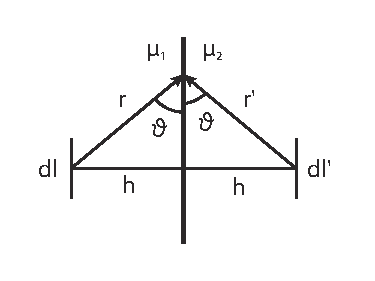
\includegraphics[width=.5\textwidth]{borderline}
\end{figure}

Направим ось \( z \) в перпендикулярно плоскости раздела сред в сторону первой
среды. Плоскость же раздела возьмем за координату \( z = 0 \).

Векторный потенциал искомого поля будем искать в виде:
\[
	\vec{A}_1 = \frac{\mu_1 I}{c} \oint \frac{d\vec{l}}{r} + k_1\frac{\mu_1 I}{c}
	\oint \frac{d\vec{l'}}{r'}; \quad
	\vec{A}_2 = k_2\frac{\mu_2 I}{c} \oint \frac{d\vec{l}}{r},
\]
где \( l' \) -- изображение контура \( l \), \( r \) и \( r' \) -- расстояние
рассматриваемой точки поля от элемента длины \( dl \) и \( dl' \).

Рассмотрим граничные условия. Первое: условие непрерывности векторного
потенциала на границе двух сред \( A_1 = A_2 \):
\[
	r = h\cos\theta; \quad r' = h\cos\theta.
\]

Подставляя в уравнение получаем:
\[
	\frac{\mu_1 I}{ch\cos\theta} \oint dl + k_1\frac{\mu_1 I}{ch\cos\theta}
	\oint dl' = \frac{\mu_2 I}{ch\cos\theta} \oint dl.
\]

В силу произвольности элемента \( dl \) и \( dl' \):
\[ 
	\mu_1 + k_1\mu_1 = k_2\mu_2.
\]

Второе: условие непрерывности нормальной производной от векторного потенциала
на границе:
\[
	\frac{1}{\mu_1}\pder{A_1}{n} + \frac{1}{\mu_2}\pder{A_2}{n} = \frac{I}{c}.
\]

Подставляя уравнения для потенциалов и учитывая произвольность элементов 
\( dl \) и \( dl' \), получаем:
\[
	k_1 + k_2 = 1.
\]

С учетом первого граничного условия получаем:
\[
	k_1 = \frac{\mu_2 - \mu_1}{\mu_2 + \mu_1}; \quad
	k_2 = \frac{2\mu_1}{\mu_1 + \mu_2}.
\]

Подставляя в векторный потенциал получаем:
\[
	\vec{A}_1 = \frac{\mu_1 I}{c} \oint \frac{d\vec{l}}{r} + 
	\left(\frac{\mu_2 - \mu_1}{\mu_2 + \mu_1}\right)
	\frac{\mu_1 I}{c} \oint \frac{d\vec{l'}}{r'}; \quad
	\vec{A}_2 = \left(\frac{2\mu_1}{\mu_1 + \mu_2}\right)
	\frac{\mu_2 I}{c} \oint \frac{d\vec{l}}{r}.
\]

Тогда поле в произвольной точке будет иметь вид:
\[
	\vec{B} = \rot\vec{A}_1 + \rot\vec{A}_2; \quad
	\vec{H} = \frac{1}{\mu_1}\rot\vec{A}_1 + \frac{1}{\mu_2}\rot\vec{A}_2.
\]

\emph{Ответ:} \( \ds \vec{B} = \rot\vec{A}_1 + \rot\vec{A}_2 \),
\( \ds \vec{H} = \frac{1}{\mu_1}\rot\vec{A}_1 + \frac{1}{\mu_2}\rot\vec{A}_2 \).
\end{document}
